\documentclass[10pt,a4paper]{article}
\usepackage[T1]{fontenc}
\usepackage[french]{babel}
\usepackage[a4paper,margin=1.75cm,headheight=14pt]{geometry}
\usepackage{amsmath,amssymb,bm,mathtools}
\usepackage{graphicx,booktabs,array}
\usepackage{xcolor}
\usepackage{enumitem}
\usepackage{fancyhdr}
\usepackage{titlesec}
\usepackage{hyperref}

\definecolor{navy}{HTML}{0B1F33}
\definecolor{teal}{HTML}{0D9488}
\definecolor{lightteal}{HTML}{E5F5F2}
\definecolor{orange}{HTML}{F28C28}
\definecolor{paleorange}{HTML}{FFF4E8}
\definecolor{muted}{HTML}{536576}
\hypersetup{colorlinks=true,linkcolor=teal,urlcolor=teal,pdftitle={Réduction de modèle pour accélérer le calcul de la dérivée topologique en magnétostatique non linéaire}}
\pagestyle{fancy}
\fancyhf{}
\lhead{\small\color{muted}Dérivée topologique en magnétostatique}
\rhead{\small\color{muted}Étude de cas 2026}
\cfoot{\color{teal}\thepage}
\setlength{\parindent}{0pt}
\setlength{\parskip}{.46em}
\setlist[itemize]{leftmargin=1.35em,itemsep=.15em,topsep=.15em}
\setlist[enumerate]{leftmargin=1.5em,itemsep=.15em,topsep=.15em}
\titleformat{\section}{\large\bfseries\color{navy}}{\thesection.}{.5em}{}
\titleformat{\subsection}{\normalsize\bfseries\color{teal}}{\thesubsection.}{.45em}{}
\titlespacing*{\section}{0pt}{.55em}{.35em}
\titlespacing*{\subsection}{0pt}{.35em}{.22em}
\newcommand{\curl}{\operatorname{curl}}
\newcommand{\R}{\mathbb{R}}
\newcommand{\dd}{\,\mathrm d}
\newcommand{\qfield}{q=\curl K}
\newcommand{\resultbox}[1]{\begin{center}\colorbox{lightteal}{\parbox{.94\linewidth}{\small #1}}\end{center}}
\newcommand{\warnbox}[1]{\begin{center}\colorbox{paleorange}{\parbox{.94\linewidth}{\small #1}}\end{center}}
\newcommand{\codecell}[1]{\textcolor{teal}{\textsf{Code reproductible : \texttt{#1}}}}
\setcounter{tocdepth}{1}

\begin{document}
\pagenumbering{roman}

\begin{titlepage}
\thispagestyle{empty}
\begin{center}
\vspace*{1.4cm}
{\color{teal}\large ÉTUDE DE CAS 2026}\par\vspace{.9cm}
{\color{navy}\Huge\bfseries Réduction de modèle pour accélérer\\[.12em]le calcul de la dérivée topologique en magnétostatique non linéaire}\par
\vspace{1.2cm}\hrule\vspace{.85cm}
{\large Benjamin Burtin \quad--\quad Louis Jamin}\par\vspace{.25cm}
{\large Émile Frotier de Bagneux}\par
\vspace{.9cm}
{\large Filière Métiers de la Recherche -- Sujet 10}\par\vspace{.15cm}
{\color{muted}Encadrants : Théodore Cherrière et Alexandre Daby-Seesaram}\par
\vfill
\begin{minipage}{.86\linewidth}
\small\color{muted}
Reproductibilité : le notebook final\_notebook.ipynb contient la chaîne complète, du maillage aux validations POD, CP et NeuROM. Le README relie les identifiants R1 à R5 du rapport aux cellules correspondantes.
\end{minipage}
\vfill
{\color{muted}19 septembre 2026}
\end{center}
\end{titlepage}
\setcounter{page}{2}

\thispagestyle{empty}
\renewcommand{\contentsname}{Plan}
\tableofcontents
\vspace{1.4em}
{\color{navy}\large\bfseries Notations}\par\vspace{.45em}
\begin{center}\small
\renewcommand{\arraystretch}{1.25}
\begin{tabular}{@{}>{$}l<{$}p{.29\linewidth}>{$}l<{$}p{.29\linewidth}@{}}
\toprule
\omega & inclusion : disque unité & b_0 & champ ambiant constant, $(B_0,0)$\\
B_R & disque de troncature, $R=24$ & B_0 & amplitude du champ ambiant\\
K & potentiel correcteur scalaire & q=\curl K & champ correcteur vectoriel\\
\mu & paramètres de l'étude & B_s & induction de saturation du fer\\
P & nombre de snapshots & N & dimension de l'espace VectorL2\\
r & rang POD & R_{\rm CP} & rang de la décomposition CP\\
\bottomrule
\end{tabular}
\end{center}
\vfill
\begin{center}
\begin{minipage}{.94\linewidth}
\small\color{muted}
Le code de reproduction est rassemblé dans un notebook unique. Les mêmes 32 points hors grille sont réutilisés pour les comparaisons POD, CP et NeuROM.
\end{minipage}
\end{center}
\newpage
\pagenumbering{arabic}

\section{Contexte et question}
En optimisation topologique, on cherche à estimer l'effet local de l'apparition d'une petite inclusion avant de modifier la géométrie complète. La dérivée topologique fournit cette information au premier ordre. Dans le cas magnétostatique étudié ici, son calcul fait intervenir un problème extérieur autour d'une inclusion de référence \cite{ganglsturm}.

Ce travail étudie un sous-problème précis : le correcteur extérieur magnétostatique non linéaire. On part d'abord de la solution $a_0$ de la machine sans inclusion. Si une inclusion doit être testée autour d'un point $z$, le champ d'induction fourni par la machine à cet endroit est
\[
\bm b_0=\curl a_0(z).
\]
Après changement d'échelle autour de $z$, le voisinage de la perturbation est remplacé par une inclusion de référence $\omega$ plongée dans un domaine extérieur. Le champ de la machine n'intervient alors plus que par sa valeur locale $\bm b_0$, considérée comme constante dans ce problème local. En principe, ce problème extérieur doit être résolu pour chaque point candidat $z$ et pour chaque scénario de matériaux. L'inclusion étant circulaire et les matériaux isotropes, on peut fixer la direction de $\bm b_0$ et faire varier son amplitude $B_0$. Le vecteur $\bm\mu$ rassemble ainsi $B_0$, les orientations d'aimantation et, selon le cas, l'induction de saturation $B_s$.

Dans une optimisation topologique, cette évaluation est répétée en de nombreux points de la machine et pour plusieurs scénarios de matériau. Une résolution éléments finis indépendante pour chaque valeur de $\bm\mu$ peut donc devenir très coûteuse. Nous cherchons précisément à diminuer ce temps de calcul grâce à la réduction de modèle, en vérifiant d'abord que la famille de solutions possède une structure suffisamment compressible et séparable.

\resultbox{La famille de champs correcteurs est-elle suffisamment compressible et séparable pour justifier une réduction paramétrique ?}

L'étude est volontairement limitée à ce problème local. Elle ne comprend ni la résolution de la physique sur la machine complète, ni l'état adjoint, ni l'évaluation finale de la dérivée topologique, ni une boucle d'optimisation. Les résultats portent sur une famille discrétisée par éléments finis et ne constituent pas encore une validation sur une machine industrielle.

\section{Problème extérieur et quantité étudiée}
\subsection{Formulation faible}
Soit $\omega$ le disque de centre $0$ et de rayon $1$, représentant l'inclusion, et $\R^2$ le domaine extérieur théorique. Le correcteur scalaire $K$ appartient à l'espace de Beppo--Levi
\[
V=\{\varphi\in H^1_{\rm loc}(\R^2):\curl\varphi\in L^2(\R^2)^2\},
\]
qui impose une énergie de champ finie ; dans le calcul tronqué, cet espace devient $H^1_0(B_R)$. Pour toute fonction test $\varphi\in V$, il vérifie
\begin{equation}\label{eq:weak}
\int_{\R^2}\curl\varphi\cdot\left[h_\omega(\bm b_0+\curl K)-h_\omega(\bm b_0)\right]\dd x
=-\int_\omega\curl\varphi\cdot\left[h_{\rm in}(\bm b_0)-h_{\rm out}(\bm b_0)\right]\dd x .
\end{equation}
Ici, $h_\omega=h_{\rm in}$ dans l'inclusion et $h_\omega=h_{\rm out}$ à l'extérieur. L'équation~\eqref{eq:weak} est le modèle local étudié ; la résolution de la machine complète sert uniquement à fournir $\bm b_0$.

\subsection{Loi constitutive}
Pour modéliser un matériau magnétique, on relie l'induction $\bm b$ au champ $\bm h$ par la loi constitutive
\[
h(\bm b)=\nu(|\bm b|)\bm b-\bm m,
\]
où $\nu$ est la reluctivité et $\bm m$ l'aimantation éventuelle. Le fer suit une loi monotone de saturation de type Marrocco \cite{marrocco},
\[
\nu(s)=\nu_{\min}+(\nu_0-\nu_{\min})f((s/B_s)^\alpha),
\]
avec $\mu_r=5000$, $B_s=1{,}9$~T et $\alpha=8$. Les calculs emploient des unités normalisées, avec $\nu_0=1$ pour le vide. Ce changement d'échelle évite qu'un critère d'arrêt absolu de Newton, mal adapté aux grandeurs SI d'ordre $10^5$, ne provoque un échec artificiel dans les cas avec aimant ; les rangs et erreurs relatives sont invariants par cette normalisation.

Quatre choix de $f$ sont comparés : rationnel, arctangente, exponentiel et algébrique. La figure~\ref{fig:laws} montre leur décrochement autour de $B_s$ et une tangente $dH/dB$ positive, condition de monotonie utilisée dans la construction énergétique. Sur la réponse du correcteur, l'écart maximal entre les trois autres lois et la loi rationnelle reste compris entre $3{,}3\%$ et $7{,}2\%$ sur la plage testée : le choix de la loi ne change pas les conclusions qualitatives. Tous les résultats de réduction utilisent ensuite la loi rationnelle. \codecell{R1\_VALIDATION}

\begin{figure}[ht]
\centering
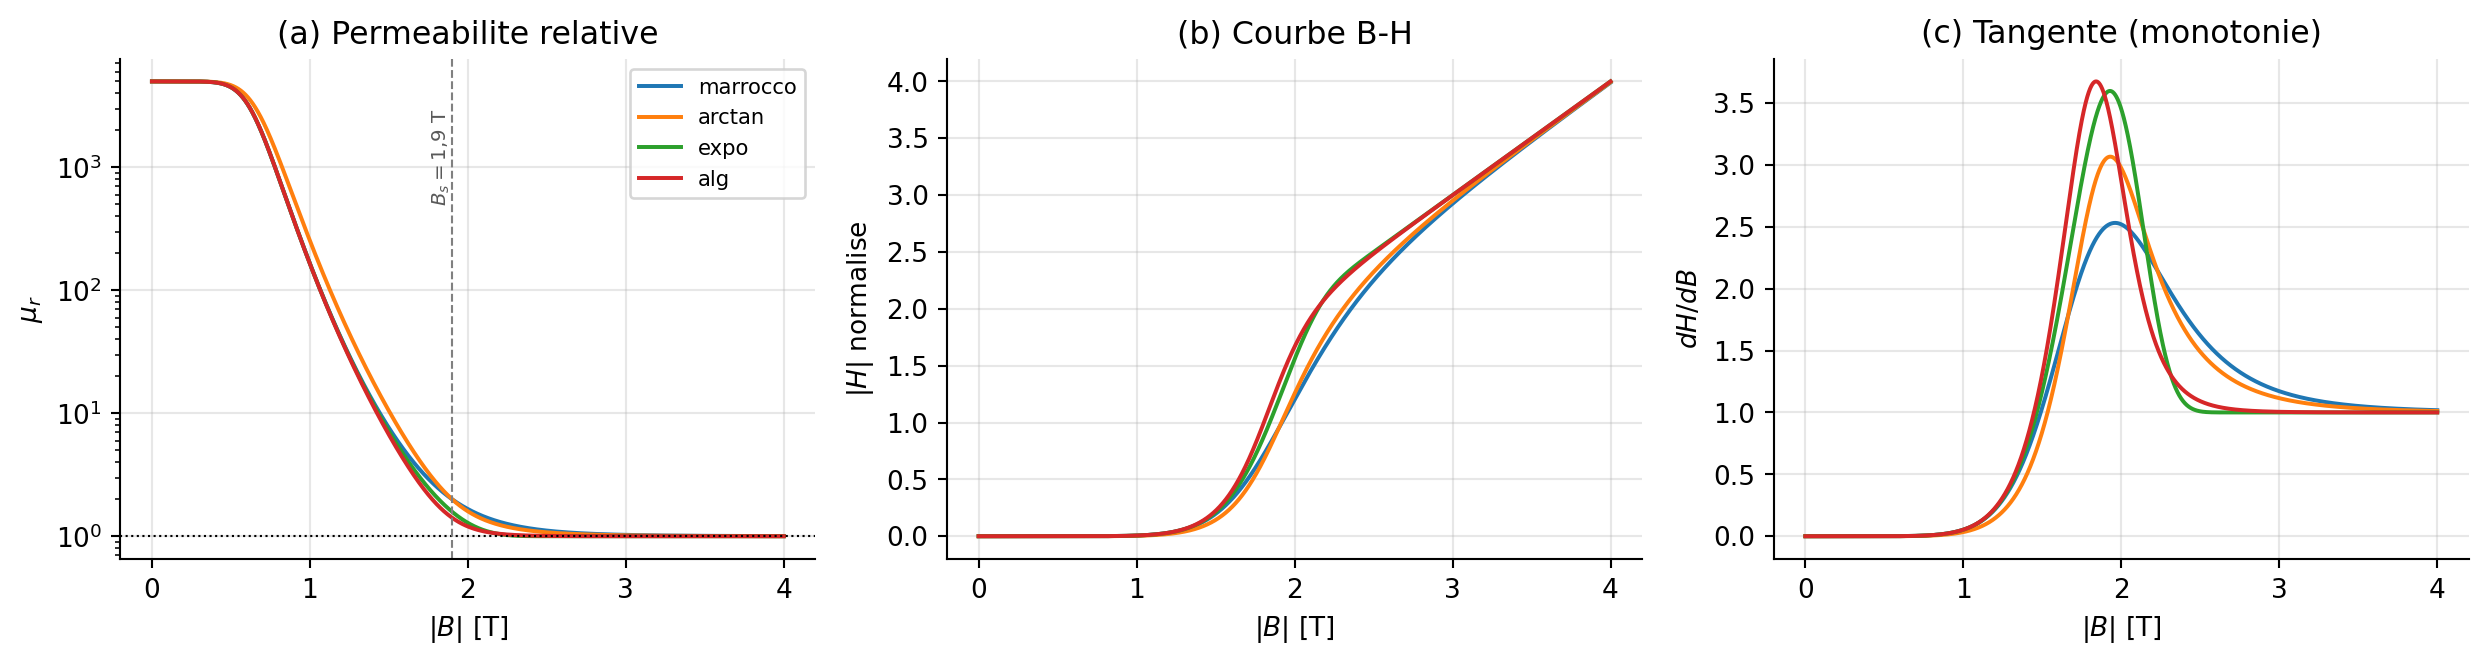
\includegraphics[width=.82\linewidth]{assets/lois_saturation.png}
\caption{Quatre lois de saturation implémentées : perméabilité relative, courbe $B$--$H$ et tangente $dH/dB$.}
\label{fig:laws}
\end{figure}

\subsection{Quantité comparée}
Le potentiel $K$ est une fonction scalaire introduite comme inconnue numérique. Ce n'est pas cette fonction que nous comparons entre paramètres : la quantité stockée et comparée est le champ vectoriel
\[
\qfield=(\partial_yK,-\partial_xK),
\]
car elle modifie directement le champ de fond dans $h$ et intervient dans la formule de la dérivée topologique. Ce choix évite de confondre une erreur de potentiel avec une erreur de champ.

La figure~\ref{fig:fields} illustre la fonction scalaire $K$ et le champ vectoriel $q$ pour une loi linéaire puis pour le fer saturé. Elle fournit aussi un contrôle visuel de la structure attendue : le potentiel présente une forme dipolaire, l'amplitude de $q$ est presque uniforme dans l'inclusion et décroît rapidement à l'extérieur, en $1/|y|^2$. La géométrie reste identique, mais les cartes d'amplitude utilisent des échelles distinctes : la saturation réduit ici l'intensité du correcteur d'environ un facteur dix. \codecell{R1\_VALIDATION}

\begin{figure}[ht]
\centering
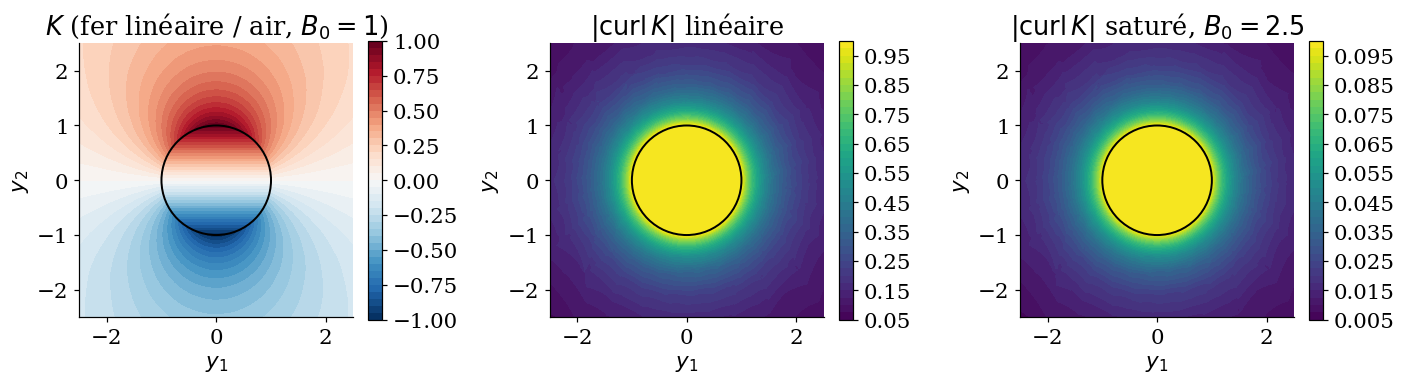
\includegraphics[width=.95\linewidth]{assets/champs.png}
\caption{Potentiel correcteur et amplitude du champ $q=\curl K$ dans les cas linéaire et saturé. Les deux cartes d'amplitude ont des échelles de couleurs distinctes : dans cette exécution, l'enveloppe passe d'environ $0,05$--$0,95$ à $0,005$--$0,095$, soit une amplitude environ dix fois plus faible.}
\label{fig:fields}
\end{figure}

\section{Discrétisation et protocole numérique}
\subsection{Maillage et troncature}
Le domaine non borné est tronqué par un disque $B_R$, avec $R=24$, et la condition $K=0$ est imposée sur son bord extérieur. La figure~\ref{fig:mesh} montre la vue globale du domaine et un zoom des éléments dans l'inclusion de rayon $1$. Le maillage comporte 484 sommets et 916 triangles, dont 132 dans l'inclusion ; il est grossier loin de $\omega$, où le correcteur devient faible, et progressivement raffiné près de l'interface. L'espace $H^1$ d'ordre 2 compte 1783 degrés de liberté après élimination des degrés imposés sur le bord. Les champs $q$ sont stockés dans un espace VectorL2 de dimension $N=5496$. Toutes les configurations partagent le même maillage afin que les colonnes d'une banque de snapshots soient comparables. La résolution éléments finis est réalisée avec NGSolve \cite{ngsolve}, et les bords circulaires sont courbés avec \texttt{mesh.Curve}.

\subsection{Contrôles de validation}
La résolution est assemblée dans NGSolve et effectuée par Newton. Trois contrôles sont utilisés : un contraste nul doit produire $q=0$, le cas linéaire est comparé à la solution analytique du disque, pour laquelle le champ moyen dans l'inclusion vaut $\alpha=(\nu_0-\nu_{\rm fer})/(\nu_0+\nu_{\rm fer})$, et la sensibilité au rayon de troncature est mesurée. Les erreurs de champ sont calculées avec la matrice de masse, aussi appelée matrice de Gram, de la base discrète $\{\boldsymbol\phi_i\}$ de VectorL2,
\[
M_{ij}=\int_{B_R}\boldsymbol\phi_i\cdot\boldsymbol\phi_j\dd x,
\]
qui définit la norme $L^2$ discrète :
\[
e_M(q,\widetilde q)=\frac{\|q-\widetilde q\|_M}{\|q\|_M},
\qquad \|q\|_M^2=q^\mathsf{T}Mq.
\]
Le contraste nul donne exactement $q=0$. À $R=24$, l'erreur relative du contrôle linéaire vaut $0,405\%$ pour Fe/Air et $1,21\times10^{-6}$ pour Air/Fe. L'erreur de troncature décroît comme $O(R^{-2})$ ; ces valeurs, très inférieures aux erreurs de réduction discutées ensuite, justifient le choix $R=24$. Fe/Air signifie que le fer est dans l'inclusion et l'air à l'extérieur ; Air/Fe inverse ces rôles, ce qui change le saut de matériau dans le membre droit de l'équation~\eqref{eq:weak}. \codecell{R1\_VALIDATION}

\subsection{Cas étudiés et grilles}
Un snapshot est le champ complet $q(\cdot;\bm\mu)$ associé à un jeu de paramètres $\bm\mu$. Le tableau~\ref{tab:grids} donne les grilles fines ; dans la notation A/B, A est l'inclusion et B le matériau extérieur. AP désigne un aimant permanent uniforme et APNL un aimant permanent à loi non linéaire. Le cas Fe($B_s$)/Air étudie explicitement l'influence de $B_s$, valeur du coude de saturation de la loi du fer. \codecell{R2\_SNAPSHOTS}

\begin{table}[ht]
\centering\small
\begin{tabular}{@{}llll@{}}
\toprule
Cas & Paramètres & Grille fine & $P$\\
\midrule
Fe/Air & $B_0$ & $9$ & 9\\
Air/Fe & $B_0$ & $9$ & 9\\
Fe($B_s$)/Air & $B_0,B_s$ & $9\times5$ & 45\\
AP/Fe & $B_0,\theta_m$ & $9\times16$ & 144\\
Fe/AP & $B_0,\theta_m$ & $9\times16$ & 144\\
APNL/APNL & $B_0,\theta_{\rm in},\theta_{\rm out}$ & $5\times8\times8$ & 320\\
\bottomrule
\end{tabular}
\caption{Configurations et nombre $P$ de résolutions éléments finis de la campagne fine.}
\label{tab:grids}
\end{table}

Les grilles sont des produits cartésiens. Les amplitudes sont échantillonnées uniformément sur $B_0\in[0{,}2;3{,}2]$ pour les cinq premiers cas et sur $B_0\in[0{,}5;3{,}0]$ pour APNL/APNL ; $B_s\in[1{,}2;3{,}2]$. Le domaine APNL/APNL est resserré car il ne comporte que cinq niveaux en $B_0$ : conserver la plage large aurait doublé le pas. Les angles sont équidistants sur $[0,2\pi)$, avec périodicité et sans doublon au point $2\pi$, identique à $0$. Ce choix déterministe facilite la comparaison et les sous-grilles emboîtées ; il ne garantit toutefois pas une couverture uniforme des zones où la solution varie le plus.

\subsection{Protocole d'ensemble}
\resultbox{Chaîne a posteriori : $P$ résolutions EF $\rightarrow$ POD $\rightarrow$ CP/PARAFAC $\rightarrow$ contrôle sur 32 points LHS. \quad
Pilote a priori : maillage NGSolve $\rightarrow$ minimisation de l'énergie par NeuROM $\rightarrow$ même contrôle hors grille.}

\begin{figure}[ht]
\centering
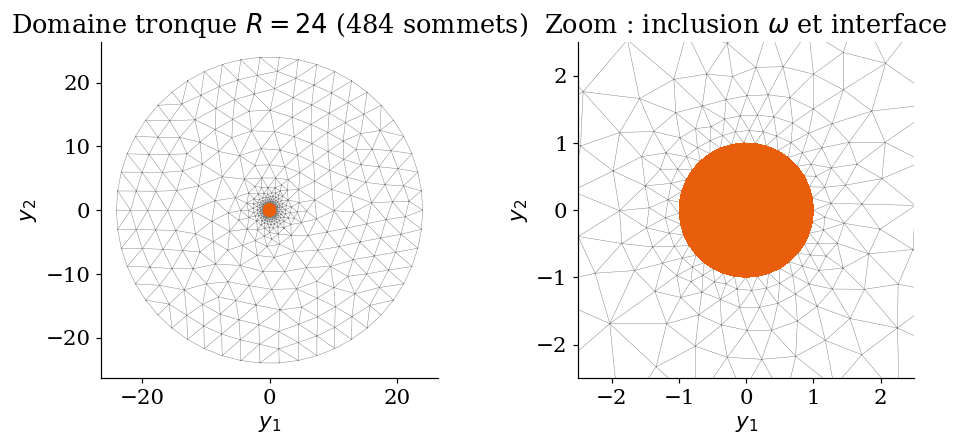
\includegraphics[width=.88\linewidth]{assets/maillage_ngsolve.png}
\caption{Maillage NGSolve : vue globale du domaine tronqué et zoom montrant les éléments dans l'inclusion et le raffinement autour de son interface.}
\label{fig:mesh}
\end{figure}

\begin{figure}[ht]
\centering
\setlength{\tabcolsep}{4pt}
\begin{tabular}{c}
\fcolorbox{teal}{lightteal}{\parbox{.72\linewidth}{\centering\small Définir les grilles d'apprentissage et les paramètres admissibles}}\\[-.1em]
$\Downarrow$\\[-.1em]
\fcolorbox{teal}{lightteal}{\parbox{.72\linewidth}{\centering\small Découper chaque axe en 32 strates et tirer une permutation avec la graine 20260916}}\\[-.1em]
$\Downarrow$\\[-.1em]
\fcolorbox{orange}{paleorange}{\parbox{.72\linewidth}{\centering\small Ajouter un décalage dans chaque strate, puis replier les angles sur $[0,2\pi)$}}\\[-.1em]
$\Downarrow$\\[-.1em]
\fcolorbox{teal}{lightteal}{\parbox{.72\linewidth}{\centering\small Réutiliser les mêmes 32 points pour POD, CP et NeuROM}}\\[-.1em]
\end{tabular}
\caption{Construction du jeu de points hors grille par hypercube latin.}
\label{fig:lhsprotocol}
\end{figure}

\section{De la POD à la séparation des paramètres}
\subsection{Deux niveaux de séparabilité}
La \emph{séparabilité espace/paramètres} cherche une somme courte $q(y;\bm\mu)\simeq\sum_{r=1}^R X_r(y)\lambda_r(\bm\mu)$ : c'est la structure mesurée par la POD. La \emph{séparabilité paramètre par paramètre} exige en plus $\lambda_r(\bm\mu)=\prod_jF_{r,j}(\mu_j)$ : c'est la contrainte imposée par CP/PARAFAC et recherchée par la PGD. La séparabilité est donc quantitative, relative à un rang, une norme et une tolérance.

\subsection{Principe et erreur de projection}
La POD diagonalise le petit Gram $S^\mathsf{T}MS$ associé à la matrice de snapshots $S$ \cite{sirovich}. Les valeurs $\sigma_j$ sont les valeurs singulières pondérées, obtenues comme racines carrées des valeurs propres de ce Gram et rangées par ordre décroissant. L'erreur relative de reconstruction moyenne sur la grille après $r$ modes est
\[
\varepsilon_{\rm POD}(r)=\sqrt{\frac{\sum_{j>r}\sigma_j^2}{\sum_j\sigma_j^2}}.
\]
Elle sépare l'espace du bloc de paramètres : les coefficients d'un mode peuvent encore dépendre conjointement de tous les paramètres. Le protocole suit quatre étapes : calcul des snapshots, POD pondérée, contrôle de la convergence lorsque $P$ augmente, puis projection de 32 nouvelles solutions hors grille.

\section{Résultats POD et convergence en nombre de snapshots}
\subsection{Deux indicateurs à ne pas confondre}
Le tableau~\ref{tab:pod} donne le premier rang $r_{2\%}$ pour lequel l'erreur moyenne de reconstruction sur les $P$ snapshots de la grille fine passe sous $2\%$. Les colonnes suivantes répondent à une autre question : à ce rang fixé, quelle est l'erreur de projection de 32 nouvelles solutions EF ? La construction de ces points est résumée par la figure~\ref{fig:lhsprotocol}.

Ces points sont tirés par hypercube latin pseudo-aléatoire avec la graine $20260916$, dans le domaine étudié et hors des noeuds d'apprentissage. Chaque axe est découpé en 32 strates de même largeur ; une permutation attribue une strate à chaque tirage et un décalage interne évite les bords. Les angles sont repliés sur $[0,2\pi)$. Le jeu est généré une seule fois et réutilisé pour les études POD, CP et NeuROM. Chaque référence POD est projetée avec ses coefficients optimaux : ce test mesure la couverture du sous-espace, pas la prédiction des coefficients à partir de $\bm\mu$. Une erreur hors grille peut donc dépasser $2\%$ sans contradiction, et ces 32 points restent un échantillon fini, pas une borne uniforme. \codecell{R3\_POD}

\begin{table}[ht]
\centering\small
\begin{tabular}{@{}lrrrrrr@{}}
\toprule
Cas & $P$ fin & $r_{2\%}$ & max & moy. & méd. & p95\\
\midrule
Fe/Air & 9 & 1 & 0,04\% & 0,03\% & 0,03\% & 0,04\%\\
Air/Fe & 9 & 4 & 6,29\% & 2,95\% & 2,35\% & 6,08\%\\
Fe($B_s$)/Air & 45 & 1 & 0,04\% & 0,02\% & 0,03\% & 0,04\%\\
AP/Fe & 144 & 20 & 10,33\% & 2,97\% & 2,64\% & 4,83\%\\
Fe/AP & 144 & 2 & 0,04\% & 0,03\% & 0,03\% & 0,04\%\\
APNL/APNL & 320 & 34 & 8,11\% & 3,25\% & 3,01\% & 6,51\%\\
\bottomrule
\end{tabular}
\caption{Rang POD à 2\% sur la grille fine et statistiques de l'erreur relative de projection sur 32 points hors grille par cas.}
\label{tab:pod}
\end{table}

\begin{figure}[ht]
\centering
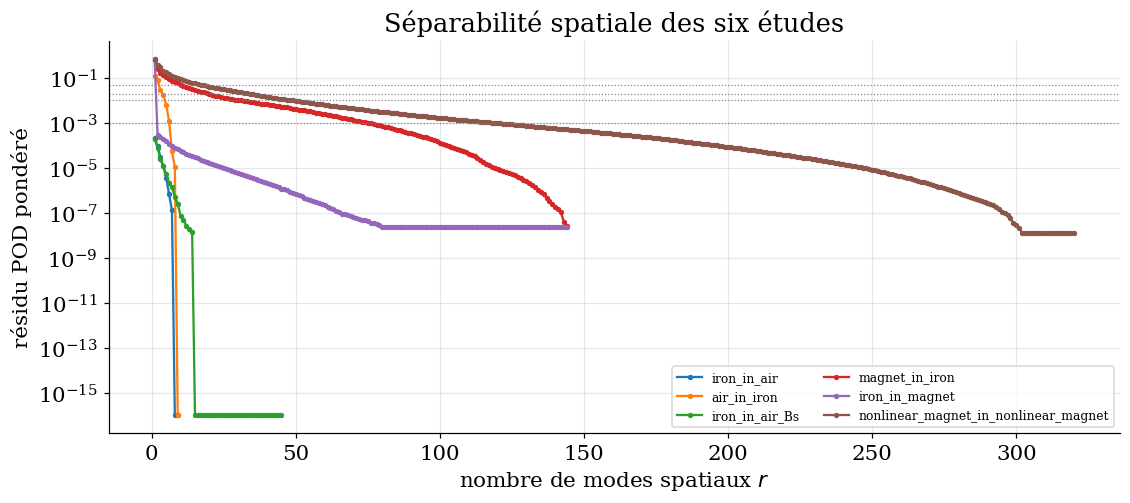
\includegraphics[width=.86\linewidth]{assets/pod_six_cas.png}
\caption{Spectres et erreurs relatives de projection POD des six configurations. Les cas riches restent compressibles, mais leur dimension augmente fortement.}
\label{fig:pod}
\end{figure}

La figure~\ref{fig:pod} et le tableau~\ref{tab:pod} montrent que quatre configurations sur six demandent au plus quatre modes à 2\%. Les familles les plus riches, AP/Fe et APNL/APNL, nécessitent 20 et 34 modes. La campagne élargie confirme une représentation très précise pour Fe/Air, Fe($B_s$)/Air et Fe/AP ; les maxima plus élevés d'Air/Fe, AP/Fe et APNL/APNL montrent l'effet conjoint de l'ordre des matériaux et de la richesse paramétrique.

\subsection{Gain de stockage}
Stocker la banque brute demande $NP$ coefficients, contre $r(N+P)$ pour les $r$ modes POD et leurs coefficients. Le facteur
\[
\frac{NP}{r(N+P)}
\]
est détaillé dans le tableau~\ref{tab:storage}.

\begin{table}[ht]
\centering\small
\begin{tabular}{@{}lrrrr@{}}
\toprule
Cas & $P$ & $r_{2\%}$ & POD $r(N+P)$ & facteur\\
\midrule
Fe/Air & 9 & 1 & 5\,505 & 9,0\\
Air/Fe & 9 & 4 & 22\,020 & 2,2\\
Fe($B_s$)/Air & 45 & 1 & 5\,541 & 44,6\\
AP/Fe & 144 & 20 & 112\,800 & 7,0\\
Fe/AP & 144 & 2 & 11\,280 & 70,2\\
APNL/APNL & 320 & 34 & 197\,744 & 8,9\\
\bottomrule
\end{tabular}
\caption{Stockage POD au seuil de 2\%, à comparer aux $NP$ coefficients de la banque brute ($N=5496$).}
\label{tab:storage}
\end{table}

Même les deux cas les plus riches gagnent un facteur voisin de 7 à 9. Air/Fe est le moins favorable : quatre modes compressent seulement neuf snapshots, donc le faible nombre de configurations limite mécaniquement le gain.

\subsection{Convergence en $P$}
\begin{figure}[ht]
\centering
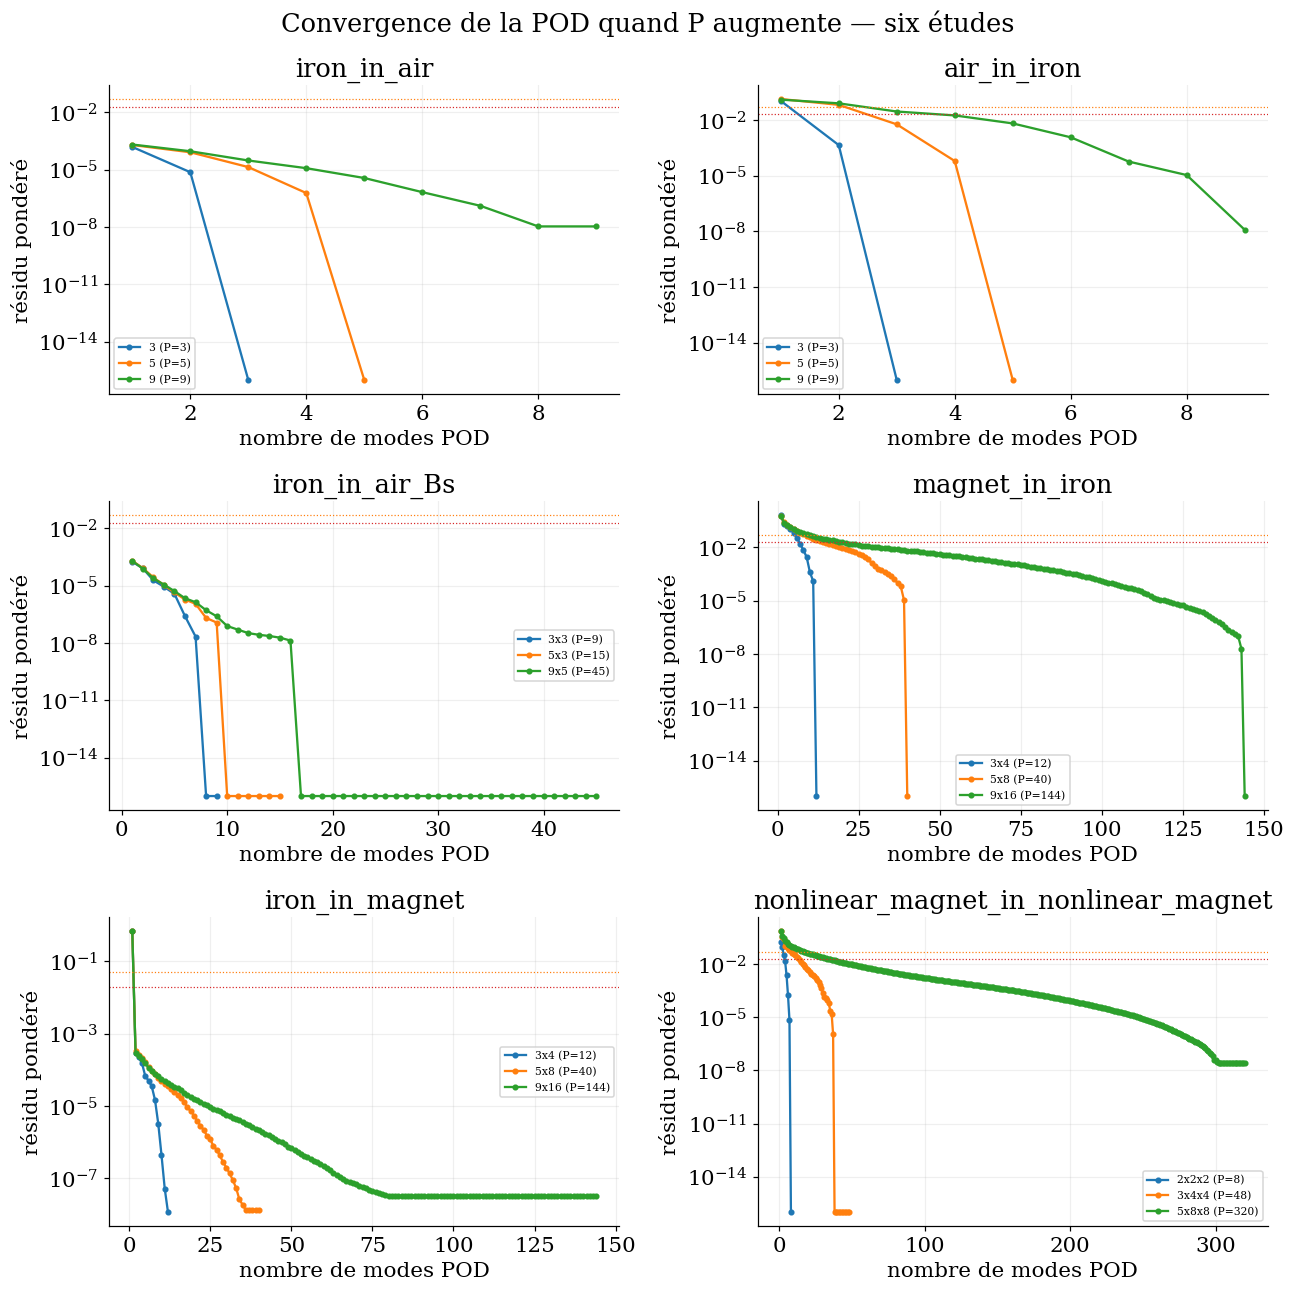
\includegraphics[width=.64\linewidth]{assets/convergence_P.png}
\caption{Influence de l'enrichissement des grilles paramétriques sur les rangs et la représentation hors grille.}
\label{fig:pconv}
\end{figure}

La figure~\ref{fig:pconv} montre que les rangs et les erreurs se stabilisent sur les derniers niveaux, alors que les premières grilles sous-estiment fortement les cas AP/Fe et APNL/APNL. Pour APNL/APNL, l'erreur hors grille passe de $97{,}8\%$ à $P=8$, à $26{,}4\%$ à $P=48$, puis à $8{,}1\%$ à $P=320$. Cette convergence en $P$ est indispensable : une grille pauvre donnerait un rang artificiellement faible. Elle reste toutefois conditionnée par le maillage spatial fixé. \codecell{R3\_POD}

\section{CP/PARAFAC sur les cas multiparamétriques}
\subsection{Reconstruction sur la grille fine}
La CP/PARAFAC réorganise les snapshots selon les axes de paramètres et cherche une représentation discrète
\[
\mathcal Q\simeq\sum_{k=1}^{R_{\rm CP}}\bm X_k\circ\bm F_k^{(1)}\circ\cdots\circ\bm F_k^{(d)},
\]
où $\circ$ désigne le produit extérieur : les composantes des vecteurs sont multipliées pour former un tenseur \cite{kolda}. Ajustée par moindres carrés alternés (ALS), elle pose une contrainte plus forte que la POD : chaque paramètre doit posséder son propre facteur. À chaque étape, un facteur est mis à jour par moindres carrés en fixant les autres. TensorLy arrête l'itération lorsque la variation absolue de l'erreur de reconstruction passe sous $\texttt{tol}=10^{-8}$, ou après 300 itérations. Le tableau indique donc soit l'arrêt selon la tolérance, soit l'atteinte de la limite de 300 itérations. Le résultat est donc un diagnostic a posteriori fondé sur les snapshots, et non une méthode qui évite leur calcul.

La figure~\ref{fig:cp} présente le balayage en rang et le tableau~\ref{tab:cp} en extrait les repères sur la grille fine. \codecell{R4\_CP}

\begin{figure}[ht]
\centering
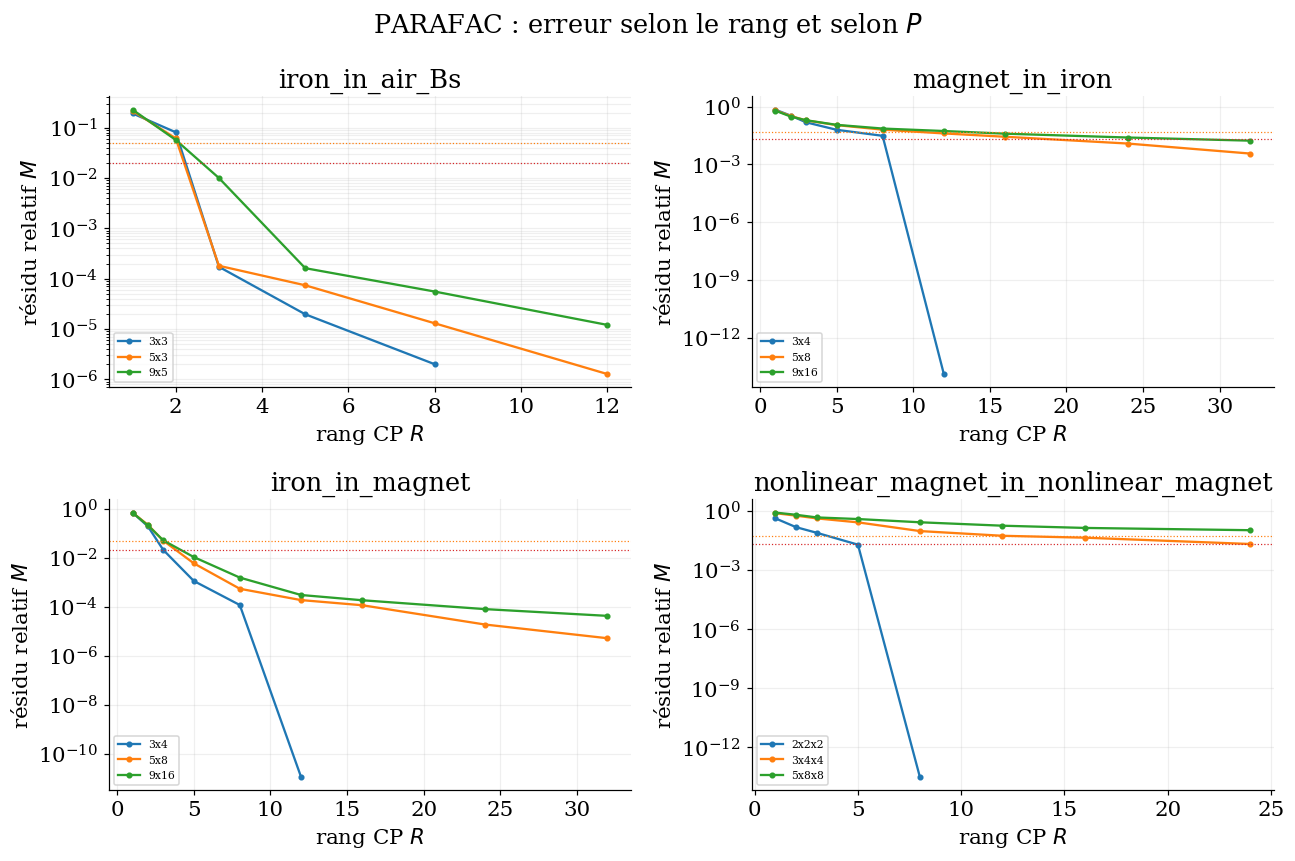
\includegraphics[width=.90\linewidth]{assets/cp_results.png}
\caption{Erreur de reconstruction CP sur les quatre cas à plusieurs paramètres. Les deux courbes difficiles restent sensibles au budget et à la stagnation d'ALS.}
\label{fig:cp}
\end{figure}

\begin{table}[ht]
\centering\small
\begin{tabular}{@{}llll@{}}
\toprule
Cas & Rang lu & Erreur CP & Arrêt ALS\\
\midrule
Fe($B_s$)/Air & $R=3$ & 1,00\% & convergence atteinte\\
AP/Fe & $R=32$ & 1,73\% & limite de 300 itérations\\
Fe/AP & $R=5$ & 1,06\% & convergence atteinte\\
APNL/APNL & $R=24$ & 10,33\% & limite de 300 itérations\\
\bottomrule
\end{tabular}
\caption{Repères de la campagne CP/ALS sur la grille fine.}
\label{tab:cp}
\end{table}

Fe($B_s$)/Air et Fe/AP présentent une forte séparabilité axe par axe sur leurs snapshots. AP/Fe reste représentable mais demande de nombreux termes et l'ALS n'est pas stabilisée au rang affiché. Pour APNL/APNL, l'erreur reste élevée à $R=24$ ; la séparation est au mieux limitée par cette campagne.

\subsection{Prédiction hors grille}
Nous testons ensuite une vraie prédiction hors grille sur les mêmes 32 points. Pour chaque facteur paramétrique CP, nous interpolons linéairement les amplitudes et périodiquement les angles. Au rang retenu (3, 32, 5 et 24), les triplets (max, moyenne, p95) valent (77,21\%, 10,07\%, 34,81\%) pour Fe($B_s$)/Air, (13,94\%, 5,05\%, 8,15\%) pour AP/Fe, (30,81\%, 2,68\%, 7,32\%) pour Fe/AP et (391,34\%, 45,06\%, 159,40\%) pour APNL/APNL. \codecell{R4\_CP}

La reconstruction CP sur grille ne garantit donc pas une interpolation stable. La décomposition est invariante par les changements d'échelle $\bm X_k\mapsto c\bm X_k$ et $\bm F_k\mapsto\bm F_k/c$ : deux noeuds voisins peuvent recevoir des facteurs d'amplitudes très différentes qui se compensent seulement dans leur produit. Interpoler séparément ces facteurs devient alors fragile. Un alignement ou une régularisation serait nécessaire, ce qui dépasse le pilote présent. Un contrôle aux noeuds d'apprentissage donne toutefois un écart maximal entre interpolation et reconstruction tensorielle inférieur à $3,7\times10^{-14}$ : le raccordement périodique et l'ordre des axes sont donc cohérents.

\section{Pilote PGD/NeuROM}
La PGD a priori \cite{chinesta} cherche directement une solution sous la forme
\[
K_R(y;\bm\mu)=\sum_{r=1}^R X_r(y)\prod_jF_{r,j}(\mu_j),
\]
en minimisant une énergie physique dont la stationnarité redonne la forme faible. Contrairement à la POD et à la CP, qui sont ici des diagnostics a posteriori fondés sur des snapshots, cette construction est a priori. Le pilote NeuROM \cite{daby} raccorde cette représentation au maillage, au curl et à la quadrature NGSolve. Adam \cite{adam} effectue une descente de gradient adaptative : il utilise des estimations de moments de premier et de second ordre des gradients pour ajuster le pas. Les produits de facteurs rendent l'optimisation non convexe, avec des symétries d'échelle (par exemple $X\mapsto cX$, $F\mapsto F/c$) et des minima ou selles dépendant de l'initialisation, même si l'énergie peut être convexe en $K$ pour une loi monotone.

\subsection{Énergie et retour à la forme faible}
L'énergie utilisée s'écrit
\begin{equation}\label{eq:energy}
\Pi_{\bm\mu}(K)=\int_{B_R}\!\left[W_{\bm\mu}(\bm b_0+\curl K)-W_{\bm\mu}(\bm b_0)-h_{\rm out}(\bm b_0)\cdot\curl K\right]\dd x,
\qquad \partial_{\bm b}W_{\bm\mu}=h_{\bm\mu}.
\end{equation}
La densité $W_{\bm\mu}$ est définie pièce par pièce dans l'intérieur et l'extérieur à partir de $h_{\rm in}$ et $h_{\rm out}$. Sur le domaine tronqué $B_R$, soustraire $W_{\bm\mu}(\bm b_0)$ ne change l'énergie que d'une constante indépendante de $K$ : le minimiseur et la formulation faible sont donc inchangés. Cette soustraction est néanmoins conservée pour normaliser $\Pi_{\bm\mu}(0)=0$ et pour obtenir l'énergie relative adaptée au domaine extérieur. En effet, lorsque $\curl K\to0$ loin de l'inclusion, l'intégrande de l'équation~\eqref{eq:energy} tend vers zéro ; sans ce terme, il tendrait vers la constante $W_{\rm out}(\bm b_0)$. L'énergie contiendrait alors un décalage proportionnel à l'aire de $B_R$, donc à $R^2$, et n'aurait pas de limite finie lorsque $R\to\infty$.

Pour vérifier l'écriture et faire apparaître explicitement le contraste de matériau, on peut aussi la développer avec $q=\curl K$ :
\begin{equation}\label{eq:energy_split}
\begin{aligned}
\Pi_{\bm\mu}(K)
={}&\int_{B_R}\!\left[W_{\rm out}(\bm b_0+q)-W_{\rm out}(\bm b_0)
-h_{\rm out}(\bm b_0)\cdot q\right]\dd x\\
&+\int_{\omega}\!\left[W_{\rm in}(\bm b_0+q)-W_{\rm out}(\bm b_0+q)
-W_{\rm in}(\bm b_0)+W_{\rm out}(\bm b_0)\right]\dd x .
\end{aligned}
\end{equation}
La somme~\eqref{eq:energy_split} est identique à~\eqref{eq:energy} : dans $\omega$, elle remplace la densité extérieure par la densité intérieure. Cette décomposition évite une ambiguïté fréquente : le terme de contraste est une différence de densités d'énergie évaluées en $\bm b_0+q$ et en $\bm b_0$, et non une constante $W_{\rm in}(\bm b_0)-W_{\rm out}(\bm b_0)$ simplement multipliée par $q$.

Pour une variation $\delta K$,
\[
\delta\Pi=\int_{B_R}\!\bigl(h_{\bm\mu}(\bm b_0+\curl K)-h_{\rm out}(\bm b_0)\bigr)\cdot\curl\delta K\dd x,
\]
et le terme entre parenthèses se décompose en
\[
h_{\bm\mu}(\bm b)-h_{\rm out}(\bm b_0)
=\bigl[h_{\bm\mu}(\bm b)-h_{\bm\mu}(\bm b_0)\bigr]
+\bigl[h_{\bm\mu}(\bm b_0)-h_{\rm out}(\bm b_0)\bigr].
\]
Le second crochet est nul hors de $\omega$ et vaut le saut $h_{\rm in}(\bm b_0)-h_{\rm out}(\bm b_0)$ dans $\omega$. La condition $\delta\Pi=0$ redonne donc exactement l'équation~\eqref{eq:weak}. Cette écriture est équivalente à la somme d'une énergie relative par matériau et du terme de contraste dans $\omega$ ; elle évite simplement deux intégrales séparées. Sa structure est commune aux trois pilotes, tandis que $W_{\rm in}$ et $W_{\rm out}$ changent avec les matériaux. \codecell{R5\_NEUROM}

\subsection{Résultats du pilote}
Les sorties exécutées avec la graine 43 donnent les repères du tableau~\ref{tab:neurom}. Les modèles sont évalués sur les mêmes 32 points hors grille que la POD et la CP. \codecell{R5\_NEUROM}

\begin{table}[ht]
\centering\small
\begin{tabular}{@{}lrrrrrr@{}}
\toprule
Cas & Rang lu & max & moy. & méd. & p95 & temps\\
\midrule
Fe/Air, $B_0$ & $R=4$ & 24,39\% & 3,20\% & 1,71\% & 8,75\% & 6,41 s\\
AP/Fe & $R=24$ & 51,52\% & 11,24\% & 7,00\% & 30,48\% & 103,70 s\\
Fe/AP & $R=12$ & 122,08\% & 7,70\% & 3,09\% & 14,05\% & 53,53 s\\
\bottomrule
\end{tabular}
\caption{Pilote NeuROM : statistiques d'erreur sur 32 points hors grille et temps d'exécution pour une initialisation donnée.}
\label{tab:neurom}
\end{table}

Pour AP/Fe, le maximum descend globalement jusqu'à 51,52\% au rang 24, mais de façon non monotone ; la médiane (7,00\%) et le p95 (30,48\%) décrivent une erreur typique bien inférieure. Pour Fe/Air, la courbe atteint un plateau après le rang 2. Les écarts périodiques entre $0$ et $2\pi$ sont nuls. Les maxima sont amplifiés lorsque la norme de référence est faible : elle vaut au pire point environ $0{,}849$ pour AP/Fe, $0{,}095$ pour Fe/AP et $0{,}062$ pour Fe/Air, contre des médianes respectives de $1{,}984$, $1{,}682$ et $0{,}795$. Cette explication est particulièrement pertinente pour Fe/AP et Fe/Air, mais ne suffit pas à expliquer le maximum AP/Fe. Le tableau~\ref{tab:neurom} démontre donc la faisabilité du raccord NGSolve/NeuROM, mais pas encore une précision compétitive.

\section{Discussion et conclusion}
Les résultats répondent positivement mais précisément à la question de départ. La famille discrétisée est compressible : quatre cas sur six atteignent 2\% d'erreur POD avec au plus quatre modes, et trois bases reproduisent les 32 points hors grille avec un maximum de 0,04\%. AP/Fe et APNL/APNL restent compressibles, mais avec des rangs 20 et 34 ; leurs maxima hors grille valent 10,33\% et 8,11\%. L'ordre des matériaux et le nombre de paramètres modifient donc fortement la richesse des champs. La présence d'angles d'aimantation semble plus pénalisante que la non-linéarité seule : une rotation se représente difficilement avec peu de modes dans une base spatiale fixe.

La CP confirme une séparabilité axe par axe nette pour Fe($B_s$)/Air et Fe/AP sur la grille connue. L'interpolation directe de ses facteurs est cependant instable : compression CP et prédiction paramétrique sont deux problèmes distincts. Pour AP/Fe, le rang élevé et la stagnation d'ALS empêchent une conclusion ferme ; pour APNL/APNL, l'erreur sur grille demeure de 10,33\% au rang 24 et l'erreur interpolée atteint 391,34\% au maximum.

Le pilote NeuROM respecte la structure spatiale-paramétrique et la périodicité, mais Adam est sensible à l'initialisation et non monotone en rang. Les erreurs maximales restent de 24,39\% pour Fe/Air, 51,52\% pour AP/Fe et 122,08\% pour Fe/AP. La prochaine étape est donc ciblée : vérifier le gradient de l'énergie par différences finies, comparer plusieurs initialisations à budget identique, puis effectuer un raffinement L-BFGS des meilleurs modèles. Ensuite seulement, une étude de convergence en maillage, en rayon $R$ et en $P$, suivie d'une comparaison des coûts hors ligne/en ligne, permettra de statuer sur l'intérêt pratique.

\resultbox{Conclusion : la réduction paramétrique est crédible pour le correcteur extérieur, avec une séparabilité particulièrement favorable dans quatre cas. CP confirme cette structure dans deux cas multiparamétriques. NeuROM est raccordé à NGSolve, mais son optimisation doit encore être fiabilisée.}

\newpage
\small
\sloppy
\begin{thebibliography}{9}
\setlength{\itemsep}{.05em}
\bibitem{ganglsturm} P. Gangl, K. Sturm. \emph{Automated computation of topological derivatives with application to nonlinear elasticity and reaction--diffusion problems}. Computer Methods in Applied Mechanics and Engineering 398, 115288 (2022). DOI: \href{https://doi.org/10.1016/j.cma.2022.115288}{10.1016/j.cma.2022.115288}.
\bibitem{marrocco} A. Marrocco. \emph{Analyse numérique de problèmes d'électrotechnique}. Ann. Sci. Math. Québec 1, 271--296 (1977).
\bibitem{ngsolve} J. Schöberl. \emph{C++11 implementation of finite elements in NGSolve}. ASC Report 30/2014, TU Wien.
\bibitem{sirovich} L. Sirovich. \emph{Turbulence and the dynamics of coherent structures. Part I}. Q. Appl. Math. 45, 561--571 (1987). DOI: \href{https://doi.org/10.1090/qam/910462}{10.1090/qam/910462}.
\bibitem{kolda} T. G. Kolda, B. W. Bader. \emph{Tensor decompositions and applications}. SIAM Review 51, 455--500 (2009). \href{https://doi.org/10.1137/07070111X}{DOI}.
\bibitem{chinesta} F. Chinesta, P. Ladevèze, E. Cueto. \emph{A short review on model order reduction based on PGD}. Arch. Comput. Methods Eng. 18, 395--404 (2011). \href{https://doi.org/10.1007/s11831-011-9064-7}{DOI}.
\bibitem{daby} A. Daby-Seesaram, K. \v{S}kardov\'a, M. Genet. \emph{Finite Element Neural Network Interpolation. Part II}. arXiv:2412.05714 (2024).
\bibitem{adam} D. P. Kingma, J. Ba. \emph{Adam: A method for stochastic optimization}. ICLR (2015), arXiv:1412.6980.
\end{thebibliography}
\fussy

\end{document}
